\documentclass{beamer}

\pdfmapfile{+sansmathaccent.map}


\mode<presentation>
{
  \usetheme{Warsaw} % or try Darmstadt, Madrid, Warsaw, Rochester, CambridgeUS, ...
  \usecolortheme{seahorse} % or try seahorse, beaver, crane, wolverine, ...
  \usefonttheme{serif}  % or try serif, structurebold, ...
  \setbeamertemplate{navigation symbols}{}
  \setbeamertemplate{caption}[numbered]
} 


%%%%%%%%%%%%%%%%%%%%%%%%%%%%
% itemize settings

\definecolor{mypink}{RGB}{255, 30, 80}
\definecolor{mydarkblue}{RGB}{60, 160, 255}
\definecolor{myblue}{RGB}{240, 240, 255}
\definecolor{mygreen}{RGB}{0, 200, 0}
\definecolor{mygreen2}{RGB}{245, 255, 230}
\definecolor{mygray}{gray}{0.8}

\setbeamertemplate{itemize items}[default]

\setbeamertemplate{itemize item}{\color{mygreen}$\blacksquare$}
\setbeamertemplate{itemize subitem}{\color{mydarkblue}$\blacktriangleright$}
\setbeamertemplate{itemize subsubitem}{\color{mygray}$\blacksquare$}



\setbeamercolor{palette quaternary}{fg=white,bg=mydarkblue}
\setbeamercolor{titlelike}{parent=palette quaternary}

\setbeamercolor{palette quaternary2}{fg=black,bg=myblue}
\setbeamercolor{frametitle}{parent=palette quaternary2}



\setbeamerfont{frametitle}{size=\Large,series=\scshape}
\setbeamerfont{framesubtitle}{size=\normalsize,series=\upshape}





%%%%%%%%%%%%%%%%%%%%%%%%%%%%
% block settings

\setbeamercolor{block title}{bg=red!30,fg=black}

\setbeamercolor*{block title example}{bg=mygreen!40!white,fg=black}

\setbeamercolor*{block body example}{fg= black,
bg= mygreen2}


%%%%%%%%%%%%%%%%%%%%%%%%%%%%
% URL settings
\hypersetup{
    colorlinks=false,
    linkcolor=blue,
    filecolor=blue,      
    urlcolor=blue,
}

%%%%%%%%%%%%%%%%%%%%%%%%%%

\renewcommand{\familydefault}{\rmdefault}

\usepackage{amsmath}
\usepackage{mathtools}


\usepackage{subcaption}

\newcommand{\bo}[1] {\mathbf{#1}}
\newcommand{\R} {\mathbb{R}}
\DeclareMathOperator*{\argmin}{arg\,min}


%%%%%%%%%%%%%%%%%%%%%%%%%%%%
% code settings

\usepackage{listings}
\usepackage{color}
% \definecolor{mygreen}{rgb}{0,0.6,0}
% \definecolor{mygray}{rgb}{0.5,0.5,0.5}
\definecolor{mymauve}{rgb}{0.58,0,0.82}
\lstset{ 
  backgroundcolor=\color{white},   % choose the background color; you must add \usepackage{color} or \usepackage{xcolor}; should come as last argument
  basicstyle=\footnotesize,        % the size of the fonts that are used for the code
  breakatwhitespace=false,         % sets if automatic breaks should only happen at whitespace
  breaklines=true,                 % sets automatic line breaking
  captionpos=b,                    % sets the caption-position to bottom
  commentstyle=\color{mygreen},    % comment style
  deletekeywords={...},            % if you want to delete keywords from the given language
  escapeinside={\%*}{*)},          % if you want to add LaTeX within your code
  extendedchars=true,              % lets you use non-ASCII characters; for 8-bits encodings only, does not work with UTF-8
  firstnumber=0000,                % start line enumeration with line 0000
  frame=single,	                   % adds a frame around the code
  keepspaces=true,                 % keeps spaces in text, useful for keeping indentation of code (possibly needs columns=flexible)
  keywordstyle=\color{blue},       % keyword style
  language=Octave,                 % the language of the code
  morekeywords={*,...},            % if you want to add more keywords to the set
  numbers=left,                    % where to put the line-numbers; possible values are (none, left, right)
  numbersep=5pt,                   % how far the line-numbers are from the code
  numberstyle=\tiny\color{mygray}, % the style that is used for the line-numbers
  rulecolor=\color{black},         % if not set, the frame-color may be changed on line-breaks within not-black text (e.g. comments (green here))
  showspaces=false,                % show spaces everywhere adding particular underscores; it overrides 'showstringspaces'
  showstringspaces=false,          % underline spaces within strings only
  showtabs=false,                  % show tabs within strings adding particular underscores
  stepnumber=2,                    % the step between two line-numbers. If it's 1, each line will be numbered
  stringstyle=\color{mymauve},     % string literal style
  tabsize=2,	                   % sets default tabsize to 2 spaces
  title=\lstname                   % show the filename of files included with \lstinputlisting; also try caption instead of title
}

%%%%%%%%%%%%%%%%%%%%%%%%%%%%
% tikz settings

\usepackage{tikz}
\tikzset{every picture/.style={line width=0.75pt}}

%%%%%%%%%%%%%%%%%%%%%%%%%%%%

\usepackage{qrcode}



\title{Discrete Dynamics}
\subtitle{Control Theory, Lecture 6}
\author{by Sergei Savin}
\centering
\date{\mydate}



\begin{document}
\maketitle


\begin{frame}{Content}

\begin{itemize}
\item Discrete Dynamics
\item Stability of the Discrete Dynamics
\item Discretization
\begin{itemize}
    \item Finite difference
    \item Finite difference in an autonomous LTI
\end{itemize}
\item Zero order hold
\item ZOH and other types of discretization
\begin{itemize}
    \item Zero order hold vs First order hold
    \item Exact discretization
\end{itemize}
\item Read more
\end{itemize}

\end{frame}





\begin{frame}{Discrete Dynamics}
% \framesubtitle{Part 1}
\begin{flushleft}

The following dynamical system is called \emph{discrete}:

\begin{equation}
    \bo{x}_{i+1} = \bo{A}\bo{x}_i + \bo{B}\bo{u}_i
\end{equation}

Note that those:

\begin{itemize}
    \item have no derivatives in the equation;
    \item are easily simulated.
\end{itemize}

\bigskip

The affine control for this system can be given as:

\begin{equation}
    \bo{u}_i = -\bo{K}\bo{x}_i + \bo{u}_i^*
\end{equation}

\end{flushleft}
\end{frame}




\begin{frame}{Stability of the Discrete Dynamics}
	\framesubtitle{Real eigenvalues}
	\begin{flushleft}
		
		Let us consider stability of the discrete dynamical system where matrix $\bo{A}$ has purely real eigenvalues:
		
		\begin{equation}
			\bo{x}_{i+1} = \bo{A}\bo{x}_i
		\end{equation}		
		
		With eigendecomposition $\bo{A} = \bo{V}^{-1} \bo{D} \bo{V}$ (where $\bo{D}$ is a diagonal matrix with eigenvalues $\lambda_j$ of $\bo{A}$ on its diagonal)  and introducing notation $\bo{z}_i = \bo{V}\bo{x}_i$ we get:
		
		\begin{equation}
			\bo{x}_{i+1} = \bo{V}^{-1} \bo{D} \bo{V}\bo{x}_i
		\end{equation}
		\begin{equation}
			\bo{z}_{i+1} =  \bo{D} \bo{z}_i
		\end{equation}
		
		Meaning that the dynamics became a system of independent scalar equations $z_{j, i+1} =  \lambda_j z_{j, i}$. 
		
		
	\end{flushleft}
\end{frame}




\begin{frame}{Stability of the Discrete Dynamics}
	\framesubtitle{Real eigenvalues}
	\begin{flushleft}
		
		Thus, with $z_{j, i+1} =  \lambda_j z_{j, i}$ we can find now the absolute value of the scalars $z_{j}$ will dwindle with time iff $|\lambda_j| < 1$:
		
		\begin{equation}
			\left| \frac{z_{j, i+1}}{z_{j, i}} \right | =   | \lambda_j |
		\end{equation}
		 
		
	\end{flushleft}
\end{frame}



\begin{frame}{Stability of the Discrete Dynamics}
	\framesubtitle{2x2 system}
	\begin{flushleft}
		
		Let us consider stability of the discrete dynamical system with a 2-by-2 matrix $\bo{A}$:
		
		\begin{equation}
			\begin{bmatrix}
				x_{1, i+1} \\ x_{2, i+1}
			\end{bmatrix}
			= 
			\begin{bmatrix}
				\alpha & -\beta \\ \beta & \alpha
			\end{bmatrix}     
			\begin{bmatrix}
				x_{1, i} \\ x_{2, i}
			\end{bmatrix}
		\end{equation}	
		
		Let us find norms of $\begin{bmatrix}
			x_{1, i+1} \\ x_{2, i+1}
		\end{bmatrix}$ and $\begin{bmatrix}
		x_{1, i} \\ x_{2, i}
	\end{bmatrix}$:


		\begin{equation}
		\left | \left|
		\begin{bmatrix}
			x_{1, i} \\ x_{2, i}
		\end{bmatrix}
		\right | \right|^2
			= 
	 	x_{1, i}^2 + x_{2, i}^2
		\end{equation}

		\begin{equation}
			\left | \left|
			\begin{bmatrix}
				x_{1, i+1} \\ x_{2, i+1}
			\end{bmatrix}
			\right | \right|^2
			= 
			(\alpha^2 + \beta^2) (x_{1, i}^2 + x_{2, i}^2)
		\end{equation}
		
		
	\end{flushleft}
\end{frame}



\begin{frame}{Stability of the Discrete Dynamics}
	\framesubtitle{2x2 system}
	\begin{flushleft}
		
		We can find the ratio of the norms of $\begin{bmatrix}
			x_{1, i+1} \\ x_{2, i+1}
		\end{bmatrix}$ and $\begin{bmatrix}
			x_{1, i} \\ x_{2, i}
		\end{bmatrix}$: 
		
		
		
		\begin{equation}
			\left | \left|
			\begin{bmatrix}
				x_{1, i+1} \\ x_{2, i+1}
			\end{bmatrix}
			\right | \right|^2 
			/ 
			\left | \left|
			\begin{bmatrix}
				x_{1, i} \\ x_{2, i}
			\end{bmatrix}
			\right | \right|^2
			= 
			\alpha^2 + \beta^2
		\end{equation}
		
		Remembering that eigenvalues of the system are $\lambda  = \alpha \pm j\beta$, we can rewrite teh expression above as:
		
		\begin{equation}
	\left | \left|
	\begin{bmatrix}
		x_{1, i+1} \\ x_{2, i+1}
	\end{bmatrix}
	\right | \right|^2 
	/ 
	\left | \left|
	\begin{bmatrix}
		x_{1, i} \\ x_{2, i}
	\end{bmatrix}
	\right | \right|^2
	= 
	| \lambda |
		\end{equation}		
		
		We can see that the norm of the variable $\bo{x}$ will dwindle with time iff $|\lambda| < 1$.
		
	\end{flushleft}
\end{frame}




\begin{frame}{Stability of the Discrete Dynamics}
\begin{flushleft}

General stability criterion is given below:

\bigskip

\begin{block}{Stability criterion}
In general, discrete systems $\bo{x}_{i+1} = \bo{A}\bo{x}_i$ are stable as long as the eigenvalues of $\bo{A}$ are smaller than 1 by absolute value: $|\lambda_i(\bo{A})| \leq 1, \; \forall i$. This is true for complex eigenvalues as well.
\end{block}


\end{flushleft}
\end{frame}



\begin{frame}{Discretization}
\framesubtitle{Finite difference}
\begin{flushleft}

Consider linear time-invariant autonomous system:

\begin{equation}
    \dot {\bo{x}} = \bo{A} \bo{x}
\end{equation}


The time derivative $\dot {\bo{x}}$ can be replaces with a finite difference:

\begin{equation}
\dot {\bo{x}} \approx \frac{1}{\Delta t}(\bo{x}(t + \Delta t) - \bo{x}(t))
\end{equation}

Note that we could have also used other definitions of a finite difference:

\begin{equation}
\dot {\bo{x}} \approx \frac{1}{\Delta t}(\bo{x}(t + 0.5\Delta t) - \bo{x}(t - 0.5\Delta t))
\end{equation}

or

\begin{equation}
\dot {\bo{x}} \approx \frac{1}{\Delta t}(\bo{x}(t) - \bo{x}(t - \Delta t))
\end{equation}

\end{flushleft}
\end{frame}




\begin{frame}{Discretization}
\framesubtitle{Finite difference notation}
\begin{flushleft}
We can introduce notation:

\begin{equation}
\begin{cases}
\bo{x}_0 = \bo{x}(0) \\
\bo{x}_1 = \bo{x}(\Delta t) \\
\bo{x}_2 = \bo{x}(2\Delta t) \\
... \\
\bo{x}_n = \bo{x}(n\Delta t) 
\end{cases}
\end{equation}

We say that $\bo{x}_i$ is the value of $\bo{x}$ at the time step $i$. Then the finite difference can be written, for example, as follows:

\begin{equation}
\dot {\bo{x}} \approx \frac{1}{\Delta t}(\bo{x}_{i+1} - \bo{x}_i)
\end{equation}

\end{flushleft}
\end{frame}



\begin{frame}{Discretization}
\framesubtitle{Finite difference in an autonomous LTI}
\begin{flushleft}

We can rewrite our original autonomous LTI as follows:

\begin{equation}
\frac{1}{\Delta t}(\bo{x}_{i + 1} - \bo{x}_i) = \bo{A} \bo{x}_i
\end{equation}
Isolating $\bo{x}_{i + 1}$ on the left hand side, we get:
\begin{equation}
\bo{x}_{i + 1} = (\bo{A} \Delta t + \bo{I}) \bo{x}_i
\end{equation}

\noindent\rule{11cm}{0.4pt}

Or alternatively:

\begin{equation}
\frac{1}{\Delta t}(\bo{x}_{i + 1} - \bo{x}_i) = \bo{A} \bo{x}_{i + 1}
\end{equation}
Isolating $\bo{x}_{i + 1}$ on the left hand side, we get:
\begin{equation}
\bo{x}_{i + 1} = (\bo{I} - \bo{A} \Delta t)^{-1} \bo{x}_i 
\end{equation}

\end{flushleft}
\end{frame}




\begin{frame}{Discretization}
\framesubtitle{Zero order hold}
\begin{flushleft}

Defining \emph{discrete state space matrix} $\bar{\bo{A}}$ and \emph{discrete control matrix} $\bar{\bo{B}}$ as follows:

\begin{equation}
\bar{\bo{A}} = \bo{A} \Delta t + \bo{I}
\end{equation}
\begin{equation}
\bar{\bo{B}} = \bo{B} \Delta t
\end{equation}
%
We get discrete dynamics:

\begin{equation}
\bo{x}_{i+1} = \bar{\bo{A}} \bo{x}_i + \bar{\bo{B}} \mathbf u_i
\end{equation}

This way of defining discrete dynamics is called \emph{zero order hold (ZOH)}.

\end{flushleft}
\end{frame}


\begin{frame}{ZOH and other types of discretization}
\framesubtitle{Zero order hold vs First order hold}
\begin{flushleft}

Graphically, we can understand what zero order hold is, by comparing it to the first order hold:

\begin{figure} [h!]
\begin{center}
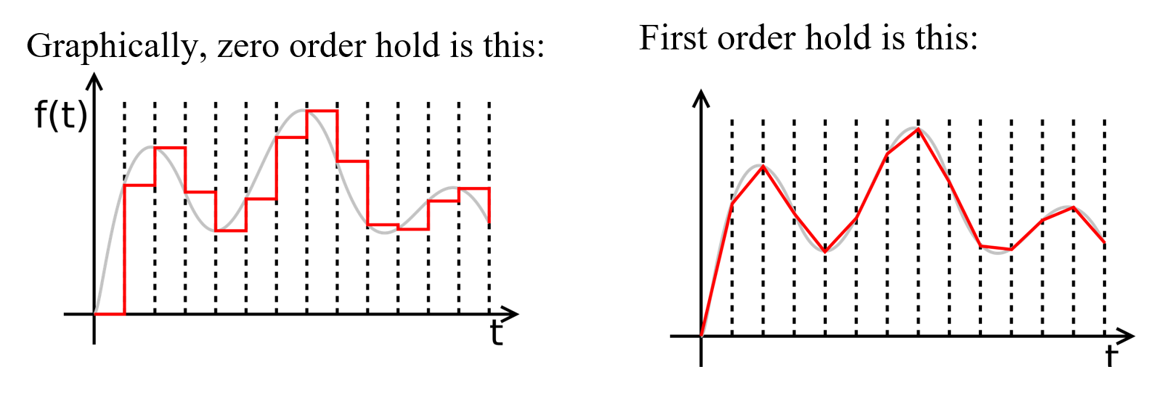
\includegraphics[width=3.5in]{ZOH.PNG}
\end{center} 
\caption{Different types of discretization} \label{F:ZOH}
\end{figure}

\end{flushleft}
\end{frame}


\begin{frame}{ZOH and other types of discretization}
\framesubtitle{Exact discretization}
\begin{flushleft}

Let the discrete state $\bo{x}_i$ correspond to continuous state $\bo{x}$ at the moment of time $t_i$. Then, we can say that the discretization is \emph{exact} the following holds for any solution $\bo{x}(t)$

\begin{equation}
\bo{x}_0 = \bo{x}(t_0) \rightarrow 
\bo{x}_i = \bo{x}(t_i), \ \forall i
\end{equation}

We can compute the exact discretization as follows:

\begin{equation}
\bar{\bo{A}} = e^{\bo{A} \Delta t}
\end{equation}
\begin{equation}
\bar{\bo{B}} = \bo{B} \int_{t_0}^{t_0 + \Delta t} e^{\bo{A} s} ds
\end{equation}


\end{flushleft}
\end{frame}












\begin{frame}{Read more}

\begin{itemize}
\item  \href{http://cse.lab.imtlucca.it/~bemporad/teaching/ac/pdf/04a-TD_sys.pdf}{Automatic Control 1 Discrete-time linear systems}, Prof. Alberto Bemporad, University of Trento


\end{itemize}

\end{frame}



\begin{frame}{Thank you!}
\centerline{Lecture slides are available via Moodle.}
\bigskip
\centerline{You can help improve these slides at:}
\centerline{\href{https://github.com/SergeiSa/Control-Theory-Slides-Spring-2021}{github.com/SergeiSa/Control-Theory-Slides-Spring-2021}}
\bigskip
\centerline{Check Moodle for additional links, videos, textbook suggestions.}
\end{frame}

\end{document}
